% Created by tikzDevice version 0.12.3 on 2020-06-04 22:28:41
% !TEX encoding = UTF-8 Unicode
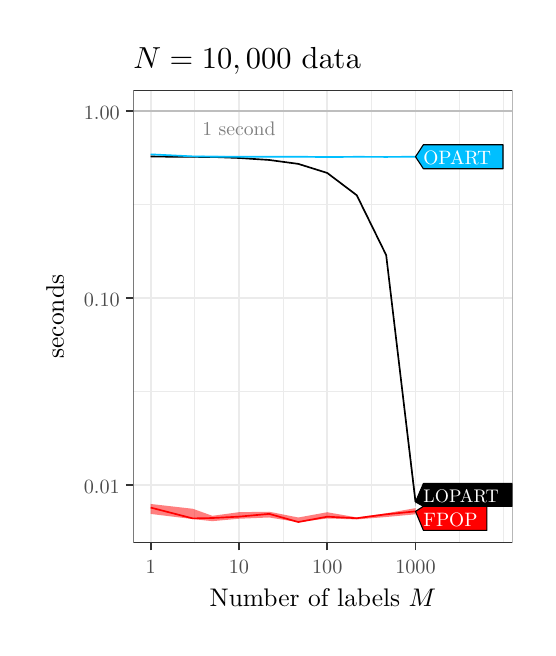
\begin{tikzpicture}[x=1pt,y=1pt]
\definecolor{fillColor}{RGB}{255,255,255}
\path[use as bounding box,fill=fillColor,fill opacity=0.00] (0,0) rectangle (180.67,216.81);
\begin{scope}
\path[clip] (  0.00,  0.00) rectangle (180.67,216.81);
\definecolor{drawColor}{RGB}{255,255,255}
\definecolor{fillColor}{RGB}{255,255,255}

\path[draw=drawColor,line width= 0.6pt,line join=round,line cap=round,fill=fillColor] (  0.00,  0.00) rectangle (180.68,216.81);
\end{scope}
\begin{scope}
\path[clip] ( 38.23, 30.69) rectangle (175.17,194.15);
\definecolor{fillColor}{RGB}{255,255,255}

\path[fill=fillColor] ( 38.23, 30.69) rectangle (175.18,194.15);
\definecolor{drawColor}{gray}{0.92}

\path[draw=drawColor,line width= 0.3pt,line join=round] ( 38.23, 85.37) --
	(175.17, 85.37);

\path[draw=drawColor,line width= 0.3pt,line join=round] ( 38.23,152.94) --
	(175.17,152.94);

\path[draw=drawColor,line width= 0.3pt,line join=round] ( 60.40, 30.69) --
	( 60.40,194.15);

\path[draw=drawColor,line width= 0.3pt,line join=round] ( 92.30, 30.69) --
	( 92.30,194.15);

\path[draw=drawColor,line width= 0.3pt,line join=round] (124.20, 30.69) --
	(124.20,194.15);

\path[draw=drawColor,line width= 0.3pt,line join=round] (156.09, 30.69) --
	(156.09,194.15);

\path[draw=drawColor,line width= 0.3pt,line join=round] (172.04, 30.69) --
	(172.04,194.15);

\path[draw=drawColor,line width= 0.6pt,line join=round] ( 38.23, 51.59) --
	(175.17, 51.59);

\path[draw=drawColor,line width= 0.6pt,line join=round] ( 38.23,119.15) --
	(175.17,119.15);

\path[draw=drawColor,line width= 0.6pt,line join=round] ( 38.23,186.72) --
	(175.17,186.72);

\path[draw=drawColor,line width= 0.6pt,line join=round] ( 44.45, 30.69) --
	( 44.45,194.15);

\path[draw=drawColor,line width= 0.6pt,line join=round] ( 76.35, 30.69) --
	( 76.35,194.15);

\path[draw=drawColor,line width= 0.6pt,line join=round] (108.25, 30.69) --
	(108.25,194.15);

\path[draw=drawColor,line width= 0.6pt,line join=round] (140.14, 30.69) --
	(140.14,194.15);
\definecolor{drawColor}{RGB}{190,190,190}

\path[draw=drawColor,line width= 0.6pt,line join=round] ( 38.23,186.72) -- (175.17,186.72);
\definecolor{drawColor}{gray}{0.50}

\node[text=drawColor,anchor=base,inner sep=0pt, outer sep=0pt, scale=  0.71] at ( 76.35,177.90) {1 second};
\definecolor{fillColor}{RGB}{255,0,0}

\path[fill=fillColor,fill opacity=0.50] ( 44.45, 44.70) --
	( 59.67, 42.96) --
	( 66.75, 40.42) --
	( 76.35, 41.73) --
	( 87.27, 41.89) --
	( 97.79, 39.81) --
	(108.25, 41.71) --
	(118.92, 39.84) --
	(129.54, 41.32) --
	(140.14, 43.20) --
	(140.14, 40.97) --
	(129.54, 39.99) --
	(118.92, 39.12) --
	(108.25, 39.46) --
	( 97.79, 38.12) --
	( 87.27, 39.82) --
	( 76.35, 39.36) --
	( 66.75, 38.49) --
	( 59.67, 39.24) --
	( 44.45, 41.10) --
	cycle;

\path[] ( 44.45, 44.70) --
	( 59.67, 42.96) --
	( 66.75, 40.42) --
	( 76.35, 41.73) --
	( 87.27, 41.89) --
	( 97.79, 39.81) --
	(108.25, 41.71) --
	(118.92, 39.84) --
	(129.54, 41.32) --
	(140.14, 43.20);

\path[] (140.14, 40.97) --
	(129.54, 39.99) --
	(118.92, 39.12) --
	(108.25, 39.46) --
	( 97.79, 38.12) --
	( 87.27, 39.82) --
	( 76.35, 39.36) --
	( 66.75, 38.49) --
	( 59.67, 39.24) --
	( 44.45, 41.10);
\definecolor{fillColor}{RGB}{0,0,0}

\path[fill=fillColor,fill opacity=0.50] ( 44.45,170.49) --
	( 59.67,170.17) --
	( 66.75,170.26) --
	( 76.35,169.72) --
	( 87.27,169.03) --
	( 97.79,167.61) --
	(108.25,164.37) --
	(118.92,156.42) --
	(129.54,134.81) --
	(140.14, 47.48) --
	(140.14, 43.83) --
	(129.54,134.63) --
	(118.92,156.12) --
	(108.25,164.26) --
	( 97.79,167.42) --
	( 87.27,168.91) --
	( 76.35,169.62) --
	( 66.75,170.00) --
	( 59.67,169.98) --
	( 44.45,170.18) --
	cycle;

\path[] ( 44.45,170.49) --
	( 59.67,170.17) --
	( 66.75,170.26) --
	( 76.35,169.72) --
	( 87.27,169.03) --
	( 97.79,167.61) --
	(108.25,164.37) --
	(118.92,156.42) --
	(129.54,134.81) --
	(140.14, 47.48);

\path[] (140.14, 43.83) --
	(129.54,134.63) --
	(118.92,156.12) --
	(108.25,164.26) --
	( 97.79,167.42) --
	( 87.27,168.91) --
	( 76.35,169.62) --
	( 66.75,170.00) --
	( 59.67,169.98) --
	( 44.45,170.18);
\definecolor{fillColor}{RGB}{0,191,255}

\path[fill=fillColor,fill opacity=0.50] ( 44.45,171.10) --
	( 59.67,170.47) --
	( 66.75,170.60) --
	( 76.35,170.26) --
	( 87.27,170.22) --
	( 97.79,170.25) --
	(108.25,170.18) --
	(118.92,170.16) --
	(129.54,170.13) --
	(140.14,170.18) --
	(140.14,170.11) --
	(129.54,170.04) --
	(118.92,170.11) --
	(108.25,170.04) --
	( 97.79,170.06) --
	( 87.27,170.07) --
	( 76.35,170.17) --
	( 66.75,170.13) --
	( 59.67,170.12) --
	( 44.45,170.76) --
	cycle;

\path[] ( 44.45,171.10) --
	( 59.67,170.47) --
	( 66.75,170.60) --
	( 76.35,170.26) --
	( 87.27,170.22) --
	( 97.79,170.25) --
	(108.25,170.18) --
	(118.92,170.16) --
	(129.54,170.13) --
	(140.14,170.18);

\path[] (140.14,170.11) --
	(129.54,170.04) --
	(118.92,170.11) --
	(108.25,170.04) --
	( 97.79,170.06) --
	( 87.27,170.07) --
	( 76.35,170.17) --
	( 66.75,170.13) --
	( 59.67,170.12) --
	( 44.45,170.76);
\definecolor{drawColor}{RGB}{255,0,0}

\path[draw=drawColor,line width= 0.6pt,line join=round] ( 44.45, 43.39) --
	( 59.67, 39.48) --
	( 66.75, 39.62) --
	( 76.35, 40.12) --
	( 87.27, 41.12) --
	( 97.79, 38.17) --
	(108.25, 40.10) --
	(118.92, 39.55) --
	(129.54, 40.97) --
	(140.14, 42.02);
\definecolor{drawColor}{RGB}{0,0,0}

\path[draw=drawColor,line width= 0.6pt,line join=round] ( 44.45,170.24) --
	( 59.67,170.11) --
	( 66.75,170.09) --
	( 76.35,169.72) --
	( 87.27,169.00) --
	( 97.79,167.59) --
	(108.25,164.31) --
	(118.92,156.25) --
	(129.54,134.64) --
	(140.14, 45.46);
\definecolor{drawColor}{RGB}{0,191,255}

\path[draw=drawColor,line width= 0.6pt,line join=round] ( 44.45,171.04) --
	( 59.67,170.30) --
	( 66.75,170.18) --
	( 76.35,170.18) --
	( 87.27,170.17) --
	( 97.79,170.18) --
	(108.25,170.05) --
	(118.92,170.15) --
	(129.54,170.10) --
	(140.14,170.17);
\end{scope}
\begin{scope}
\path[clip] ( 38.23, 30.69) rectangle (175.17,194.15);
\definecolor{drawColor}{RGB}{0,0,0}
\definecolor{fillColor}{RGB}{255,0,0}

\path[draw=drawColor,line width= 0.4pt,line join=round,line cap=round,fill=fillColor] (140.14, 42.02) --
	(142.99, 43.85) --
	(165.94, 43.85) --
	(165.94, 35.17) --
	(142.99, 35.17) --
	cycle;
\definecolor{fillColor}{RGB}{0,0,0}

\path[draw=drawColor,line width= 0.4pt,line join=round,line cap=round,fill=fillColor] (140.14, 45.46) --
	(142.99, 52.09) --
	(175.18, 52.09) --
	(175.18, 43.85) --
	(142.99, 43.85) --
	cycle;
\definecolor{fillColor}{RGB}{0,191,255}

\path[draw=drawColor,line width= 0.4pt,line join=round,line cap=round,fill=fillColor] (140.14,170.17) --
	(142.99,174.51) --
	(171.76,174.51) --
	(171.76,165.83) --
	(142.99,165.83) --
	cycle;
\definecolor{drawColor}{RGB}{255,255,255}

\node[text=drawColor,anchor=base west,inner sep=0pt, outer sep=0pt, scale=  0.70] at (142.99, 36.62) {FPOP};

\node[text=drawColor,anchor=base west,inner sep=0pt, outer sep=0pt, scale=  0.66] at (142.99, 45.22) {LOPART};

\node[text=drawColor,anchor=base west,inner sep=0pt, outer sep=0pt, scale=  0.70] at (142.99,167.28) {OPART};
\definecolor{drawColor}{gray}{0.20}

\path[draw=drawColor,line width= 0.6pt,line join=round,line cap=round] ( 38.23, 30.69) rectangle (175.18,194.15);
\end{scope}
\begin{scope}
\path[clip] (  0.00,  0.00) rectangle (180.67,216.81);
\definecolor{drawColor}{gray}{0.30}

\node[text=drawColor,anchor=base east,inner sep=0pt, outer sep=0pt, scale=  0.73] at ( 33.28, 48.56) {0.01};

\node[text=drawColor,anchor=base east,inner sep=0pt, outer sep=0pt, scale=  0.73] at ( 33.28,116.12) {0.10};

\node[text=drawColor,anchor=base east,inner sep=0pt, outer sep=0pt, scale=  0.73] at ( 33.28,183.69) {1.00};
\end{scope}
\begin{scope}
\path[clip] (  0.00,  0.00) rectangle (180.67,216.81);
\definecolor{drawColor}{gray}{0.20}

\path[draw=drawColor,line width= 0.6pt,line join=round] ( 35.48, 51.59) --
	( 38.23, 51.59);

\path[draw=drawColor,line width= 0.6pt,line join=round] ( 35.48,119.15) --
	( 38.23,119.15);

\path[draw=drawColor,line width= 0.6pt,line join=round] ( 35.48,186.72) --
	( 38.23,186.72);
\end{scope}
\begin{scope}
\path[clip] (  0.00,  0.00) rectangle (180.67,216.81);
\definecolor{drawColor}{gray}{0.20}

\path[draw=drawColor,line width= 0.6pt,line join=round] ( 44.45, 27.94) --
	( 44.45, 30.69);

\path[draw=drawColor,line width= 0.6pt,line join=round] ( 76.35, 27.94) --
	( 76.35, 30.69);

\path[draw=drawColor,line width= 0.6pt,line join=round] (108.25, 27.94) --
	(108.25, 30.69);

\path[draw=drawColor,line width= 0.6pt,line join=round] (140.14, 27.94) --
	(140.14, 30.69);
\end{scope}
\begin{scope}
\path[clip] (  0.00,  0.00) rectangle (180.67,216.81);
\definecolor{drawColor}{gray}{0.30}

\node[text=drawColor,anchor=base,inner sep=0pt, outer sep=0pt, scale=  0.73] at ( 44.45, 19.68) {1};

\node[text=drawColor,anchor=base,inner sep=0pt, outer sep=0pt, scale=  0.73] at ( 76.35, 19.68) {10};

\node[text=drawColor,anchor=base,inner sep=0pt, outer sep=0pt, scale=  0.73] at (108.25, 19.68) {100};

\node[text=drawColor,anchor=base,inner sep=0pt, outer sep=0pt, scale=  0.73] at (140.14, 19.68) {1000};
\end{scope}
\begin{scope}
\path[clip] (  0.00,  0.00) rectangle (180.67,216.81);
\definecolor{drawColor}{RGB}{0,0,0}

\node[text=drawColor,anchor=base,inner sep=0pt, outer sep=0pt, scale=  0.92] at (106.70,  7.64) {Number of labels $M$};
\end{scope}
\begin{scope}
\path[clip] (  0.00,  0.00) rectangle (180.67,216.81);
\definecolor{drawColor}{RGB}{0,0,0}

\node[text=drawColor,rotate= 90.00,anchor=base,inner sep=0pt, outer sep=0pt, scale=  0.92] at ( 13.08,112.42) {seconds};
\end{scope}
\begin{scope}
\path[clip] (  0.00,  0.00) rectangle (180.67,216.81);
\definecolor{drawColor}{RGB}{0,0,0}

\node[text=drawColor,anchor=base west,inner sep=0pt, outer sep=0pt, scale=  1.10] at ( 38.23,202.22) {$N=10,000$ data};
\end{scope}
\end{tikzpicture}
